\documentclass{article}
\usepackage{amsmath, amsthm}
\usepackage{listings, xcolor}
\usepackage{graphicx}

\title{Report to Project-2}
\author{Yuanbo Han\quad15300180032}
\date{November 19, 2017}

\graphicspath{{figures/}}

\lstset{
columns=fixed,
numbers=left,
frame=none,
keywordstyle=\color[RGB]{40,40,255},
numberstyle=\footnotesize\color{darkgray},
commentstyle=\it\color[RGB]{0,96,96},
stringstyle=\rmfamily\slshape\color[RGB]{128,0,0},
showstringspaces=false,
language=Matlab,
}

\newcommand \w{\mathbf{w}}
\newcommand \x{\mathbf{x}}
\newcommand \xxi{\mathbf{x}^{(i)}}
\newcommand \yi{y^{(i)}}
\newcommand \sumi {\sum_{i=1}^}

\begin{document}
\maketitle

\tableofcontents


\section{Logistic Regression}
\subsection{Bayes' Rule}
\begin{align*}
p(y=1|x) &= \frac{p(x|y=1)p(y=1)}{p(x|y=1)p(y=1)+p(x|y=0)p(y=0)} \\
&= \frac{ \frac{\alpha}{(2\pi)^\frac{D}{2} \left| \Sigma^\frac{1}{2} \right|}
e^{-\frac{1}{2} (x-\mu_1)^T \Sigma^{-1} (x-\mu_1)} }
{ \frac{\alpha}{(2\pi)^\frac{D}{2} \left| \Sigma^\frac{1}{2} \right|}
e^{-\frac{1}{2} (x-\mu_1)^T \Sigma^{-1} (x-\mu_1)}
+ \frac{1-\alpha}{(2\pi)^\frac{D}{2} \left| \Sigma^\frac{1}{2} \right|}
e^{-\frac{1}{2} (x-\mu_0)^T \Sigma^{-1} (x-\mu_0)} } \\
&= \frac{1}{1+\frac{1-\alpha}{\alpha}
e^{-\frac{1}{2} \left[ (x-\mu_0)^T \Sigma^{-1}(x-\mu_0) - (x-\mu_1)^T \Sigma^{-1}(x-\mu_1) \right] } } \\
&= \frac{1}{1+\frac{1-\alpha}{\alpha}
e^{-\frac{1}{2} \sumi{D} \frac{1}{\sigma_i^2} \left[ (x_i-\mu_{i0})^2 - (x_i-\mu_{i1})^2 \right] } } \\
&= \frac{1}{1+\frac{1-\alpha}{\alpha}
e^{-\frac{1}{2} \sumi{D} \frac{1}{\sigma_i^2} \left[ 2(\mu_{i1}-\mu_{i0})x + \mu_{i0}^2 - \mu_{i1}^2 \right] } } \\
&= \frac{1}{1 + e^{-\sumi{D} \frac{\mu_{i1}-\mu_{i0}}{\sigma_i^2}x_i
- \left( \sumi{D} \frac{\mu_{i0}^2 - \mu_{i1}^2}{2\sigma_i^2} - \log \frac{1-\alpha}{\alpha} \right) } } \\
\end{align*}
Let $w_i = \frac{\mu_{i1}-\mu_{i0}}{\sigma_i^2}$,
$\w = (w_1, w_2, \cdots, w_D)^T$,
$b = \sumi{D} \frac{\mu_{i0}^2-\mu{i1}^2}{2\sigma_i^2} - \log \frac{1-\alpha}{\alpha}$,
then
\[
p(y=1|x) = \frac{1}{ 1+e^{-\w^Tx-b} } = \sigma \left( \w^Tx+b \right)
\]

\subsection{Maximum Likelihood Estimation}
\begin{align*}
E(\w, b) &= - \sumi{N} \log p\left( \yi | \xxi \right) \\
&= - \sumi{N} \left\{ \yi \log p\left( y=1 | \xxi \right) + \left( 1 - \yi \right) \log p\left( y=0 | \xxi \right) \right\} \\
&= - \sumi{N} \left\{ \yi \log \frac{p\left(y=1|\xxi \right)}{p\left(y=0|\xxi \right)} + \log p\left( y=0 | \xxi \right) \right\} \\
&= - \sumi{N} \left\{ \left( \yi-1 \right) \left( {\xxi}^T\w + b \right) - \log \left( 1 + e^{-{\xxi}^T\w - b} \right) \right\}
\end{align*}
If we write
\begin{align*}
\mathbf{X} &= \left[ \begin{array}{ccccc}
x_1^{(1)} & x_2^{(1)} & \cdots & x_D^{(1)} & 1  \\
x_1^{(2)} & x_2^{(2)} & \cdots & x_D^{(2)} & 1  \\
\vdots & \vdots & \ddots & \vdots & \vdots  \\
x_1^{(N)} & x_2^{(N)} & \cdots & x_D^{(N)} & 1
\end{array} \right]  \\
y &= \left( y^{(1)}, y^{(2)}, \cdots, y^{(N)} \right)^T
\end{align*}
and
\[
\mathbf{W} = (w_1, w_2, \cdots, w_D, b)^T
\]
then
\begin{align}
E(\w, b) &= -\mathbf{W}^T \mathbf{X}^T (y-1) - \sumi{N} \log \sigma \left( \mathbf{X} \mathbf{W} \right)  \\
\frac{\partial E(\w, b)}{\partial \mathbf{W}} &=  -\mathbf{X}^T \left( y - \sigma \left( \mathbf{X} \mathbf{W} \right) \right)
\end{align}

\subsection{L2 Regularization}
\begin{align*}
p(\mathcal{D} | \w, b) &= \prod_{i=1}^N p\left( \yi | \xxi, \w, b \right) \\
&= e^{\sumi{N} \log p\left( \yi | \xxi, \w, b \right)} \\
&= e^{-E(\w, b)} \\
p(\w, b) &= \prod_{i=1}^N \mathcal{N} \left( w_j | 0, \frac{1}{\lambda} \right) \cdot \mathcal{N} \left( b | 0, \frac{1}{\lambda} \right) \\
&= \frac{1}{(2\pi)^\frac{D+1}{2} \left( \frac{1}{\lambda} \right)^\frac{D+1}{2}}
e^{-\frac{1}{2} \sum_{j=1}^D \frac{w_j^2}{\frac{1}{\lambda}} - \frac{1}{2} \frac{b^2}{\frac{1}{\lambda}}} \\
&= \left( \frac{\lambda}{2\pi} \right)^\frac{D+1}{2} e^{-\frac{\lambda}{2} \left( \sum_{j=1}^D w_j^2 + b^2 \right)}
\end{align*}
By Bayes' rule,
\begin{align*}
p(\w, b | \mathcal{D}) &= \frac{p(\mathcal{D} | \w, b) p(\w,b)}{p(\mathcal{D})} \\
&\propto p(\mathcal{D} | \w, b) p(\w, b) \\
&=\left( \frac{\lambda}{2\pi} \right)^\frac{D+1}{2} e^{-E(\w, b)-\frac{\lambda}{2} \left( \sum_{j=1}^D w_j^2 + b^2 \right)} \\
L(\w, b) &= -log \left\{ \left( \frac{\lambda}{2\pi} \right)^\frac{D+1}{2}
e^{-E(\w, b)-\frac{\lambda}{2} \left( \sum_{j=1}^D w_j^2 + b^2 \right)} \right\} \\
&= E(\w, b) + \frac{\lambda}{2} \sum_{j=1}^D w_j^2 + \frac{\lambda}{2} b^2 + C(\lambda)
\end{align*}
where $C(\lambda) = \frac{D+1}{2} \log \frac{2\pi}{\lambda}$.


\section{Digit Classification}
\subsection{k-Nearest Neighbors}
The script $knn\_plot.m$ written by me runs kNN for different values of $k \in \{1, 3, 5, 7, 9\}$, and plots the classification rate on the validation set as a function of k (see Figure~1).

\begin{figure}
\centering
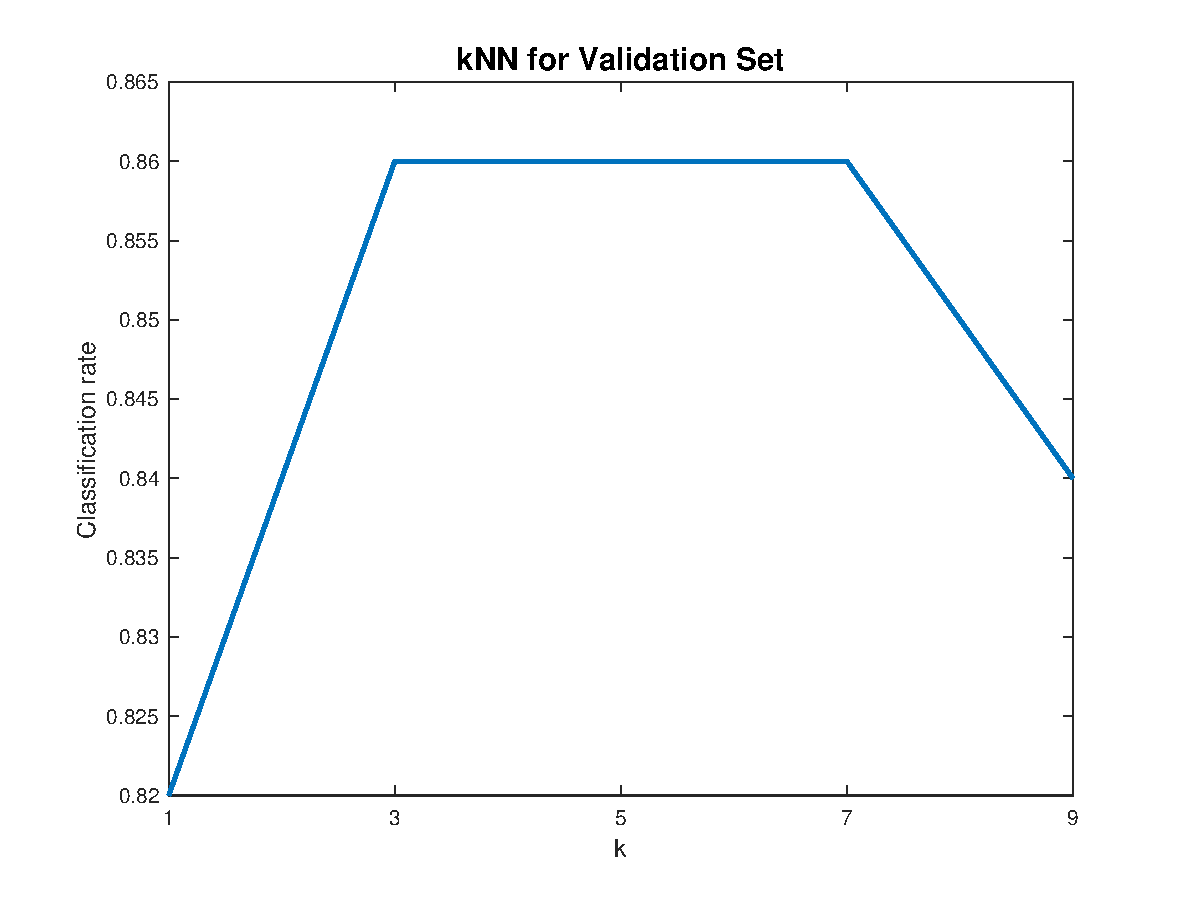
\includegraphics[scale=0.4]{1.eps}
\caption{Classification rate against k}
\end{figure}

As we can see in the figure, $k=3,5,7$ performs the best, so the final $k$ we will choose is among them. Since $5$ is in the middle  of $\{3,5,7\}$, we can infer that $k=5$ is more steady to perform well than $k=3$ or $k=7$. Therefore, I'd like to choose $k^\star=5$, and the classification rate on the test set is 94\%. For comparison, I write $plot\_knn.m$ to compute the rate for $k^\star-2=3$ and $k^\star+2=7$ as well, and plot them in Figure~2.

As a consequence, the outcome agrees with my analysis.

\begin{figure}
\centering
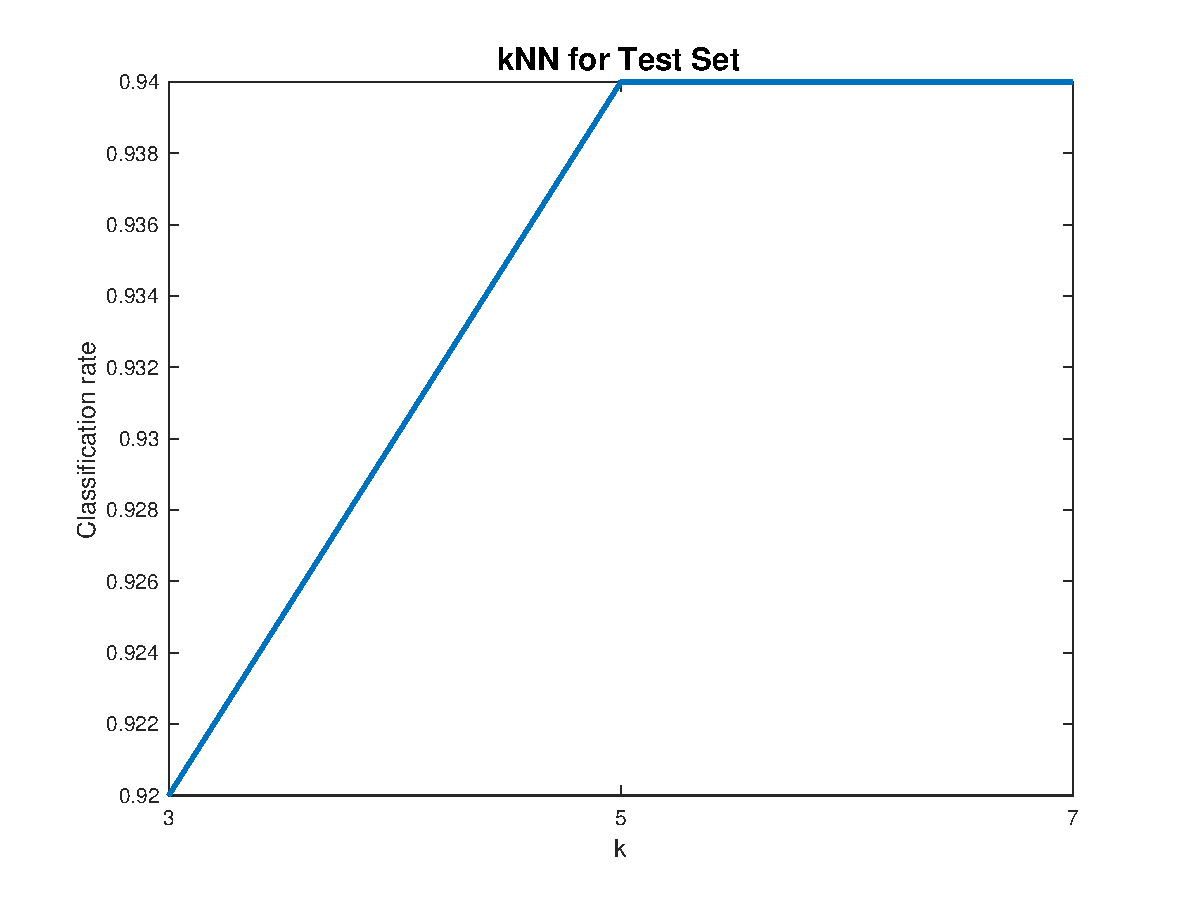
\includegraphics[scale=0.4]{2.eps}
\caption{Comparison among my chosen $k^\star$, $k^\star-2$ and $k^\star+2$}
\end{figure}

\subsection{Logistic Regression}
Codes of $logistic.m$, $logistic\_predict.m$ and $evaluate.m$ are in the Appendix.

It is necessary to mention that, in the original provided script\\$logistic\_regression\_template.m$, the learning rate is actually\\$\frac{hyperparameters.learning\_rate}{N}$, where $N$ is the number of examples in training data. However, I found no good to do this division, and it is even troublesome when comparing performance of different training sets. Since $N$ remains a constant once we have chosen a certain training set, we can simply delete it and use $hyperparameters.learning\_rate$ as the true learning rate. Through the whole experiment below, I have applied $hyperparameters.learning\_rate$ instead of $\frac{hyperparameters.learning\_rate}{N}$, and I will not mention this again.

From my experiment, it performs well to set\\$hyperparameters.learning\_rate=0.001$, $hyperparameters.num\_iterations = 300$, and initialize $weights$ randomly by standard normal distribution. Running it once on the test set, the final stats is 
\begin{lstlisting}
ITERATION: 300   NLOGL: 0.05
TRAIN_CE:0.054999 TRAIN_FRAC:99.38
VALIC_CE:0.432754 VALID_FRAC:88.00
TEST_CE:0.294021 TEST_FRAC:88.00
\end{lstlisting}

My script $plot\_cross\_entropy.m$ shows how the cross entropy changes as training progresses. The result is in Figure~3.
\begin{figure}
\centering
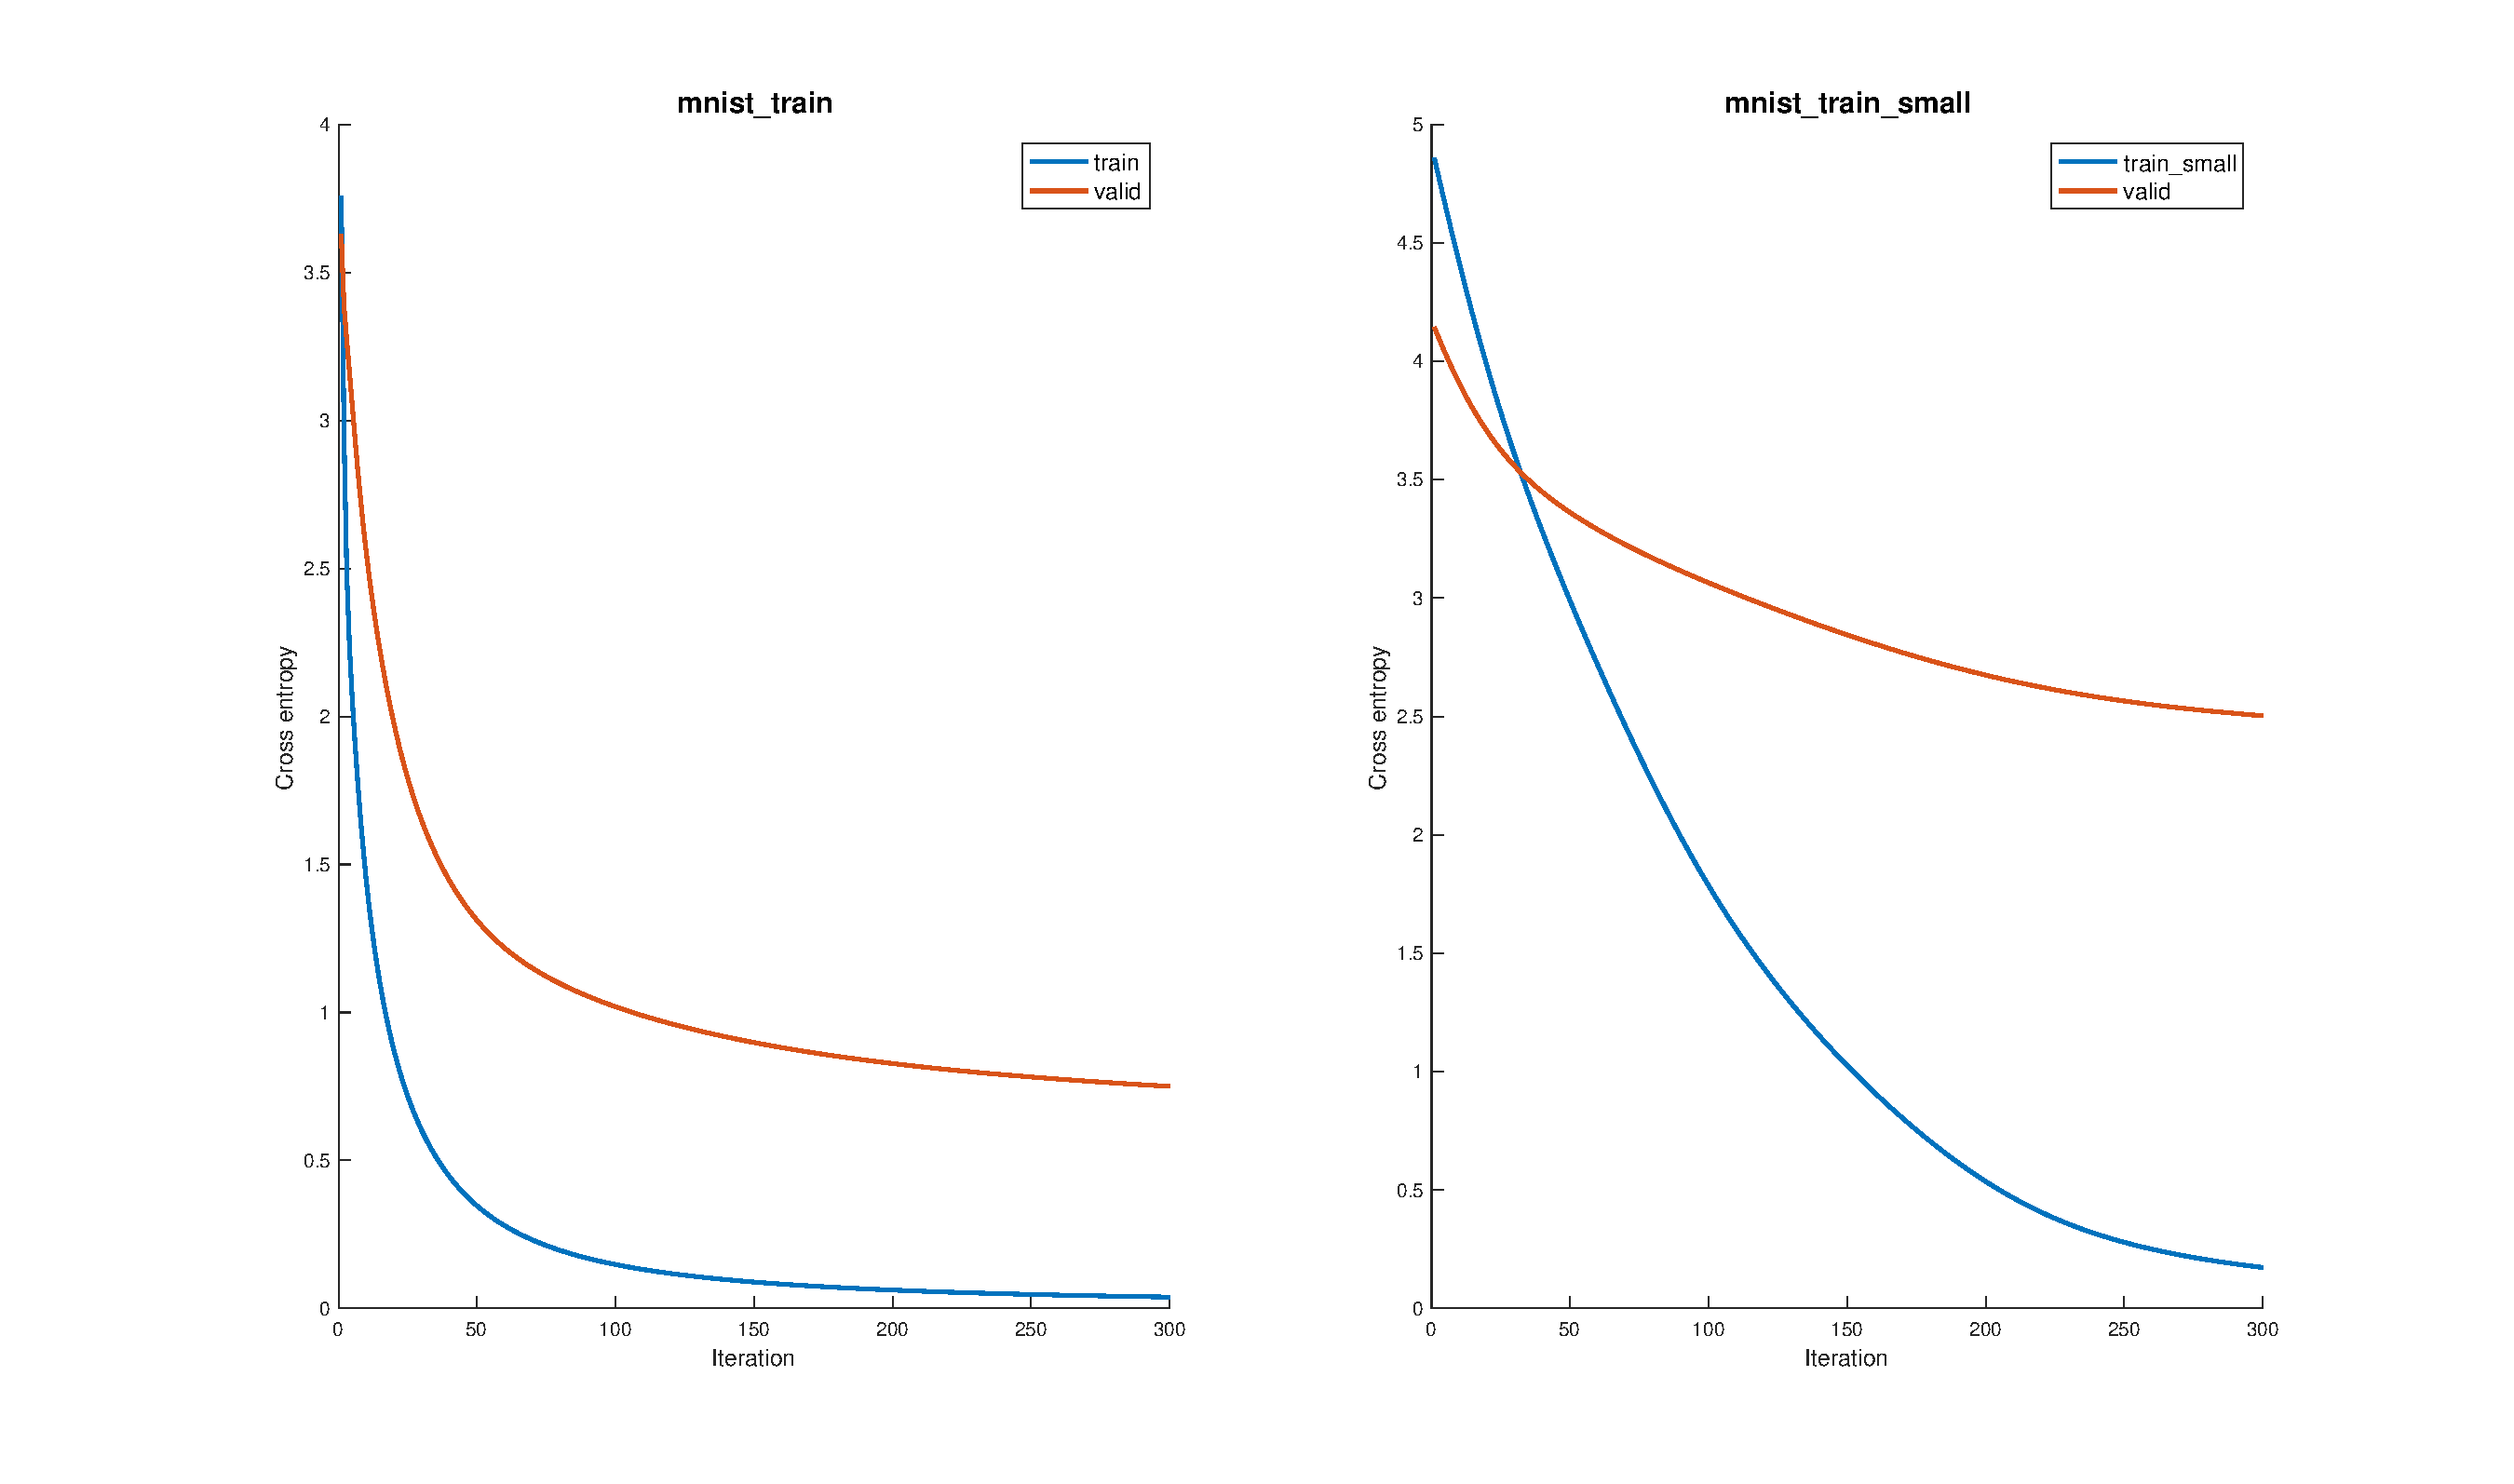
\includegraphics[scale=0.25]{3.eps}
\caption{Cross entropy as training progresses}
\end{figure}

Running $plot\_cross\_entropy.m$, the plot does change subtly. That is mainly because the initial $weights$ is set randomly. In practical experiment, I first fix all the initial values of weight parameters to be $0$. Then I run the program and change $hyperparameters.learning\_rate$ and $hyperparameters.num\_iterations$ several times to make them ideal. And finally I let $weights$ randomly initialized by standard normal distribution, which proves to perform well.

\subsection{Penalized Logistic Regression}
Codes of $logistic\_pen.m$ are in the Appendix.
My $plot\_stats\_against\_lambda.m$ plots the average cross entropy and classification rate against $\lambda$. The result is in Figure~4.
\begin{figure}
\centering
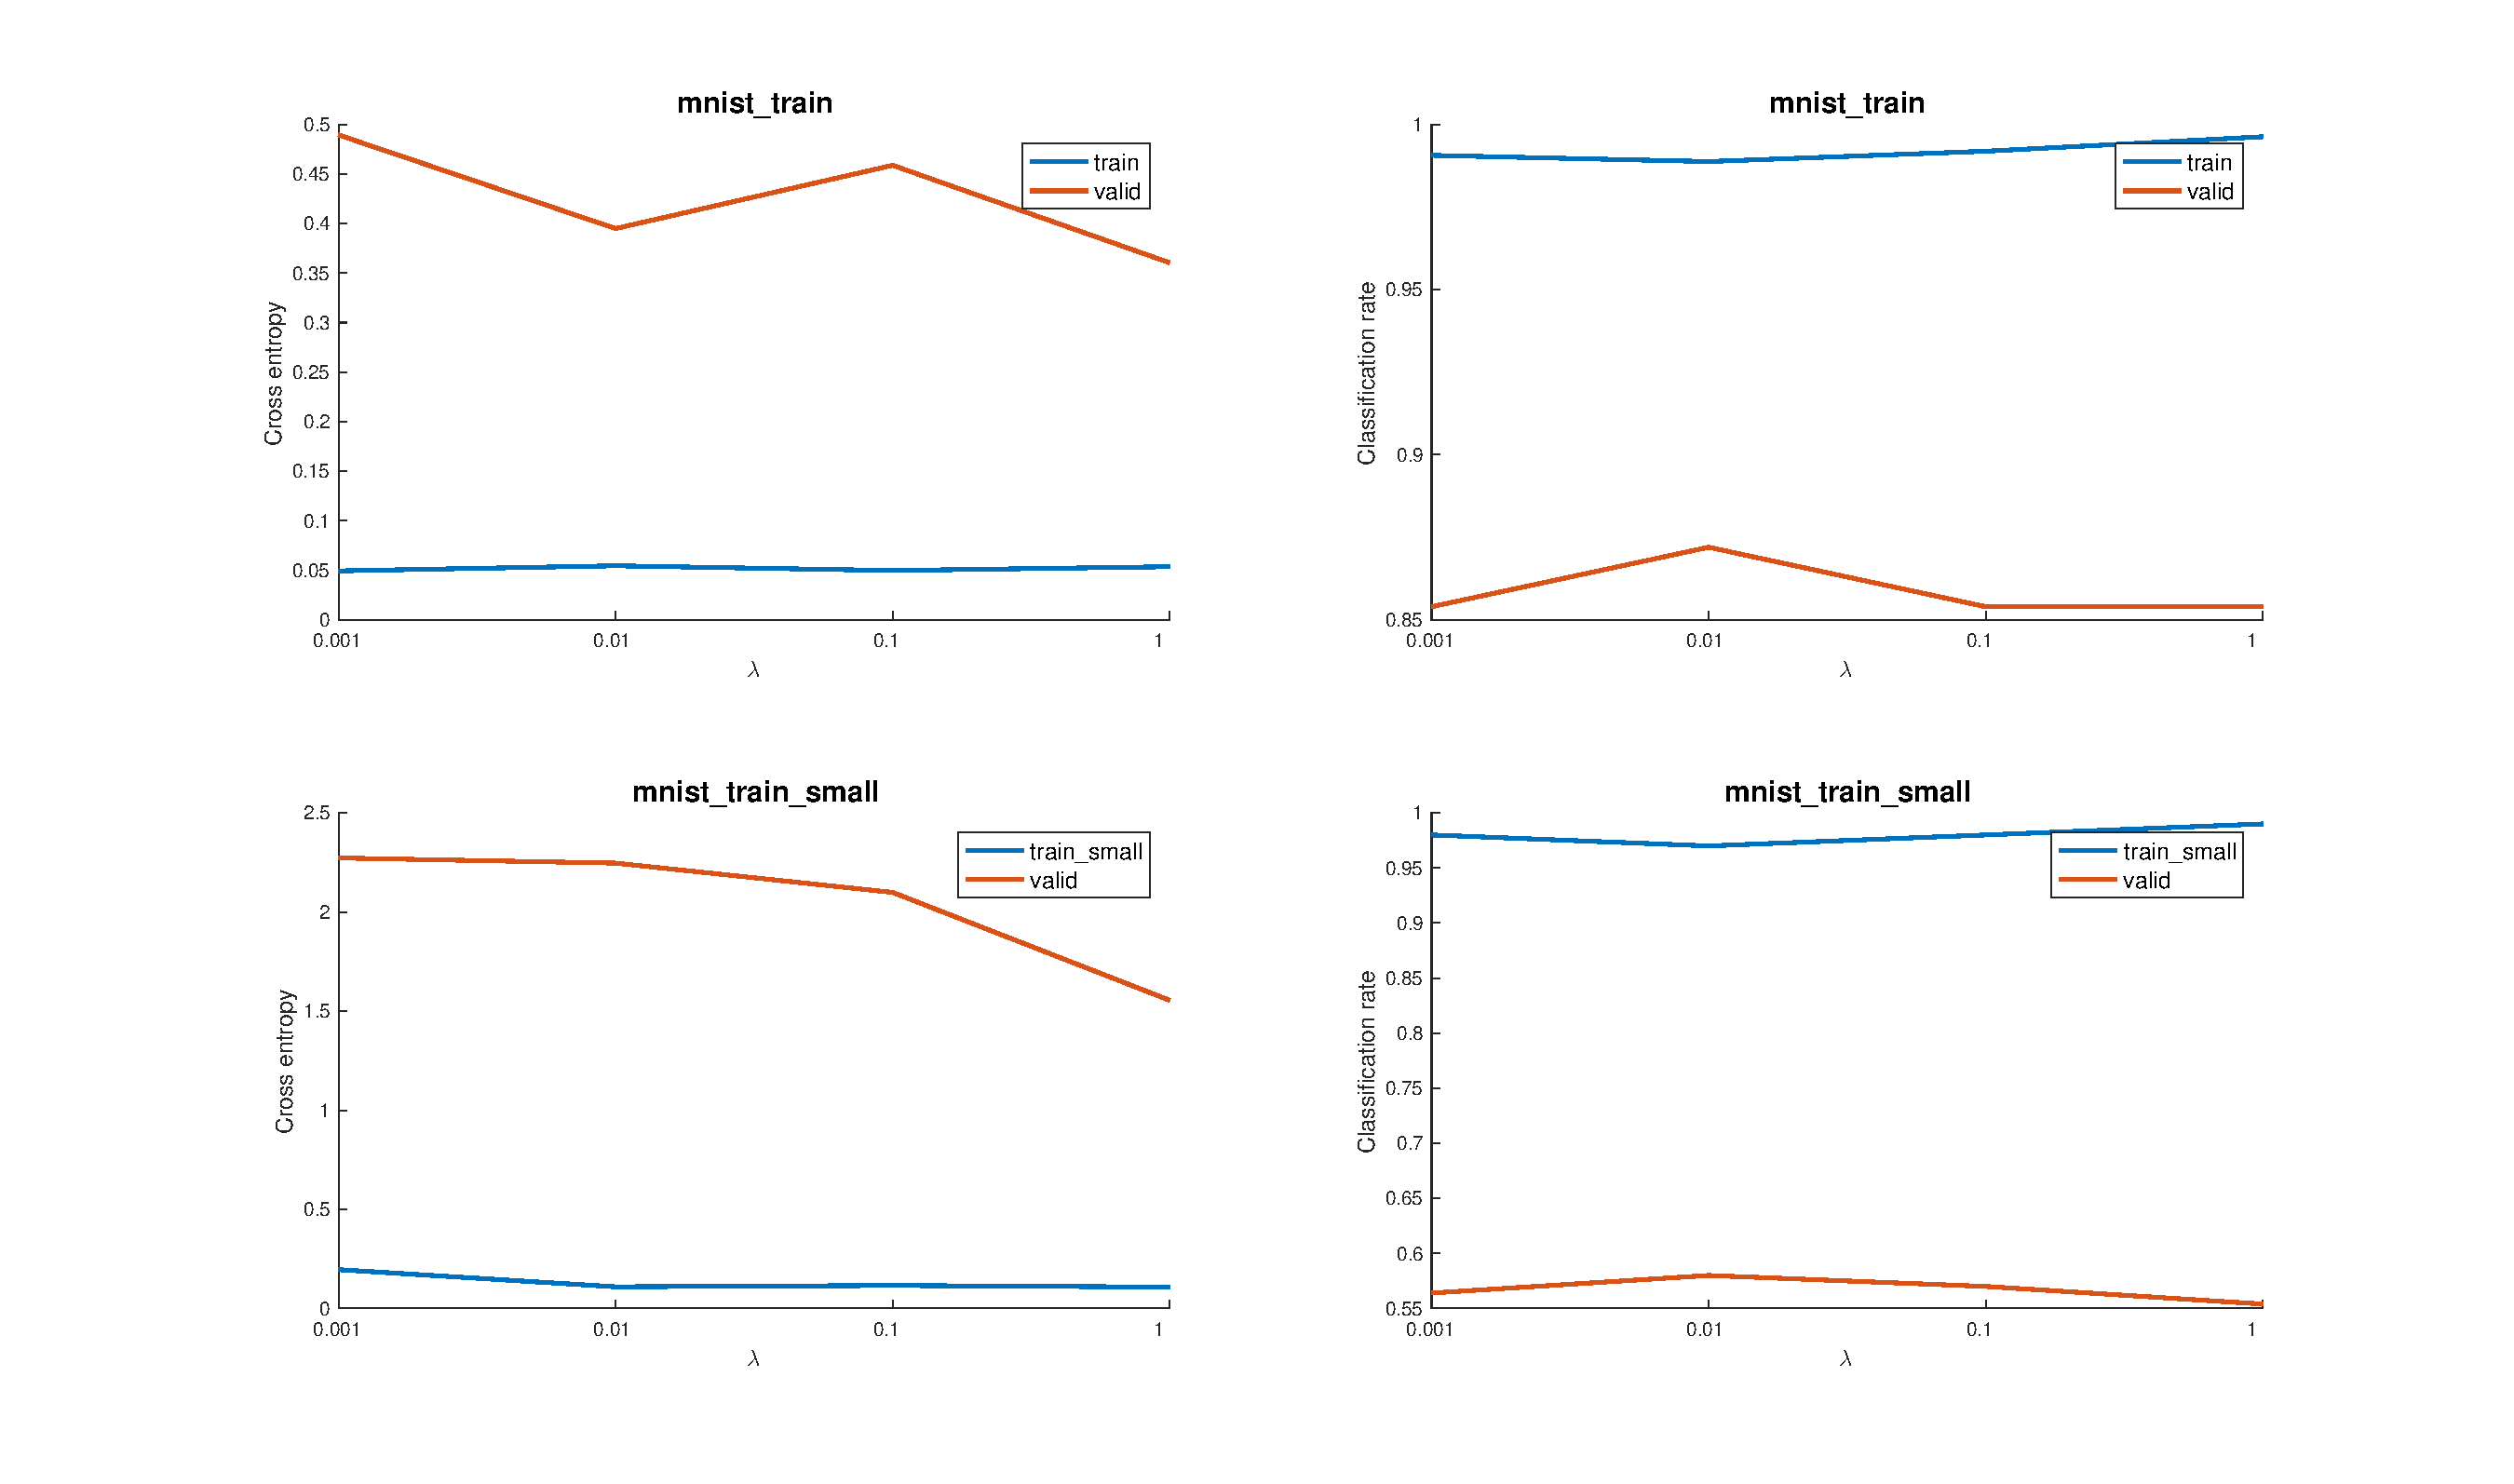
\includegraphics[scale=0.25]{4.eps}
\caption{Average cross entropy and classification rate against $\lambda$}
\end{figure}
The best $\lambda$ for both training sets is $\lambda=0.01$, since the average classification rates of valid data is the highest with $\lambda=0.01$. And in this situation, the classification rate of test data is 92\% for $mnist\_train$ and 70\% for $mnist\_train\_small$.

For explanation, a small $\lambda$ is exactly what we want, for it reduces the influence of those unimportant parameters of $weights$. That's why it performs bad when $\lambda$ is big. However, a quite small $\lambda$ is too near to $0$, and it will be similar to the situation without penalty.

\subsection{Naive Bayes}
The implementation is $run\_nb.m$ in the Appendix. The result is in Figure~5.

The visualization of the mean and variance vectors for both classes look respectively like 4s and 9s. The difference is that the visualization for the mean fades from the inner to the outer, but that for the variance fades from the outer to the inner.
\begin{figure}
\centering
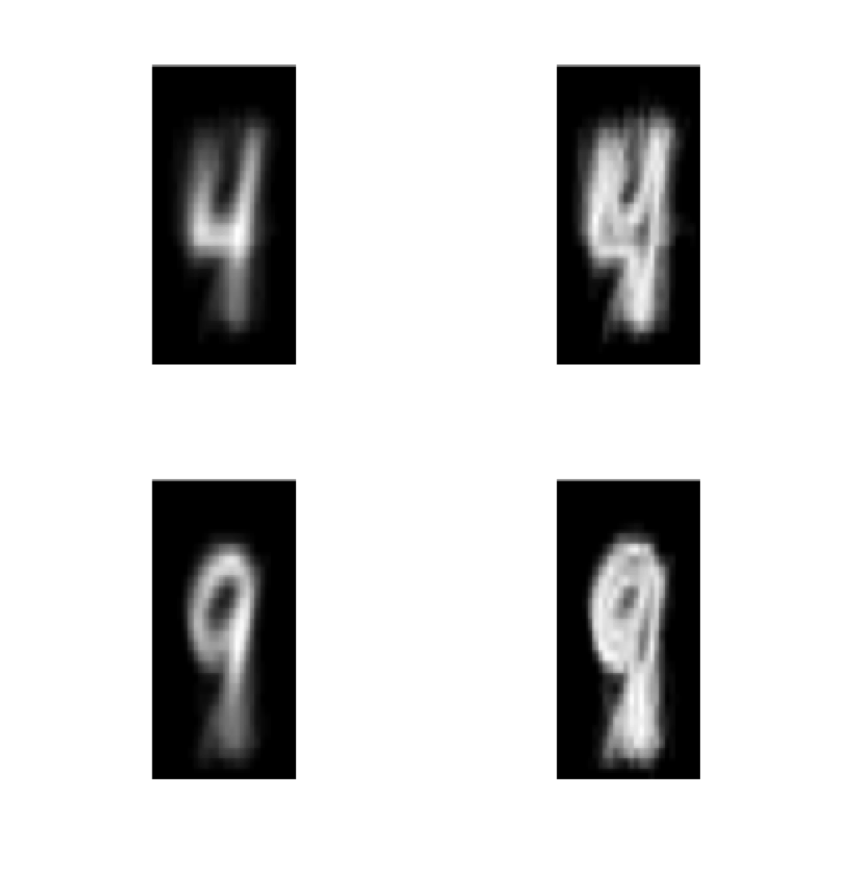
\includegraphics[scale=0.4]{5.png}
\caption{Visualization of the mean and variance vectors}
\end{figure}

\subsection{Compare k-NN, Logistic Regression, and Naive Bayes}
The Naive Bayes classifier is the simplest method but performs the worst. k-NN has to choose a right k to perform well, while it is still easy to achieve. The logistic regression is the most complicated method among these three, especially when we add penalty. There are at least 3 kinds of parameters for us to modify. But of course, it pays off with the highest classification rate.

\section{Stochastic Subgradient Methods}
\subsection{Averaging Strategy}
Codes of $svmAvg.m$ are in the Appendix. The result is in Figure~6.
\begin{figure}
\centering
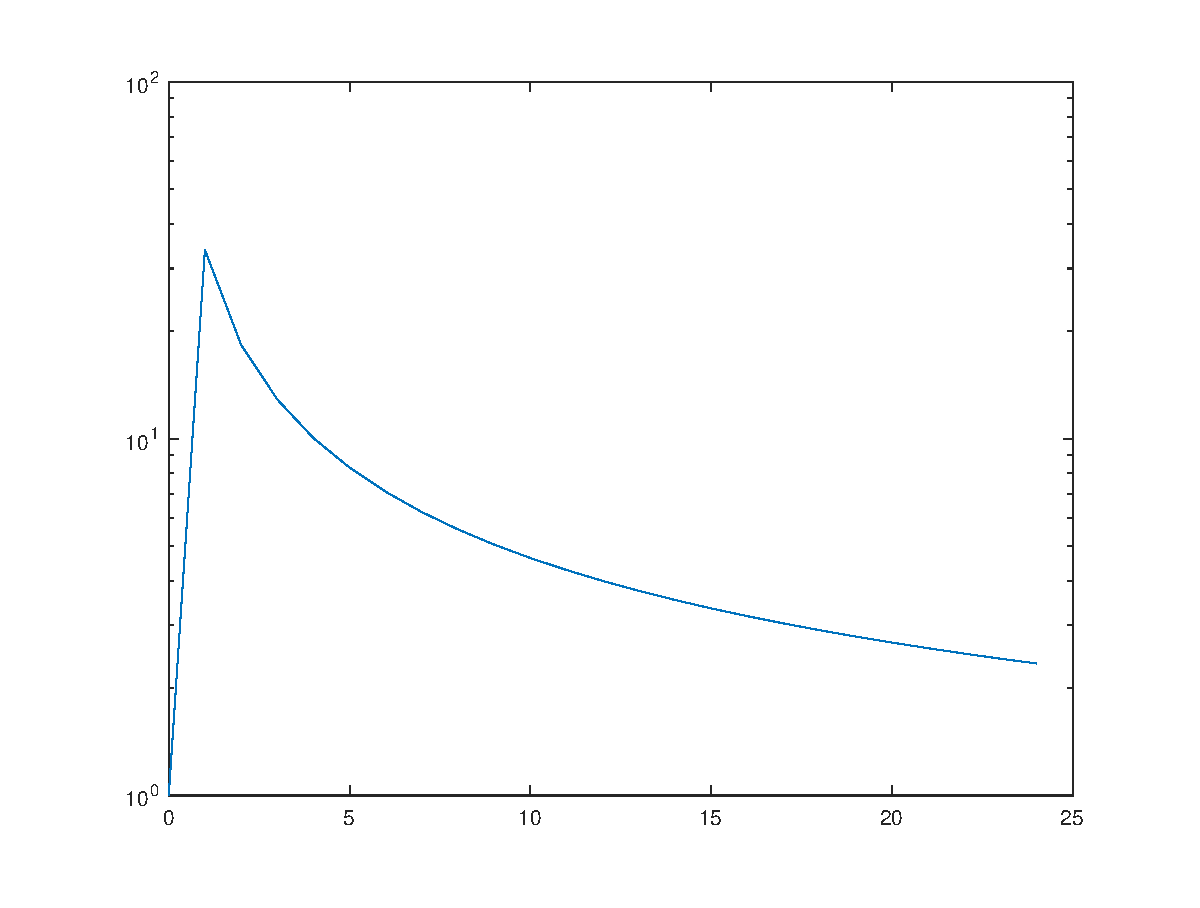
\includegraphics[scale=0.4]{6.eps}
\caption{svmAvg}
\end{figure}

\subsection{Second-Half Averaging Strategy}
Codes of $svmHalfAvg.m$ are in the Appendix. The result is in Figure~7.
\begin{figure}
\centering
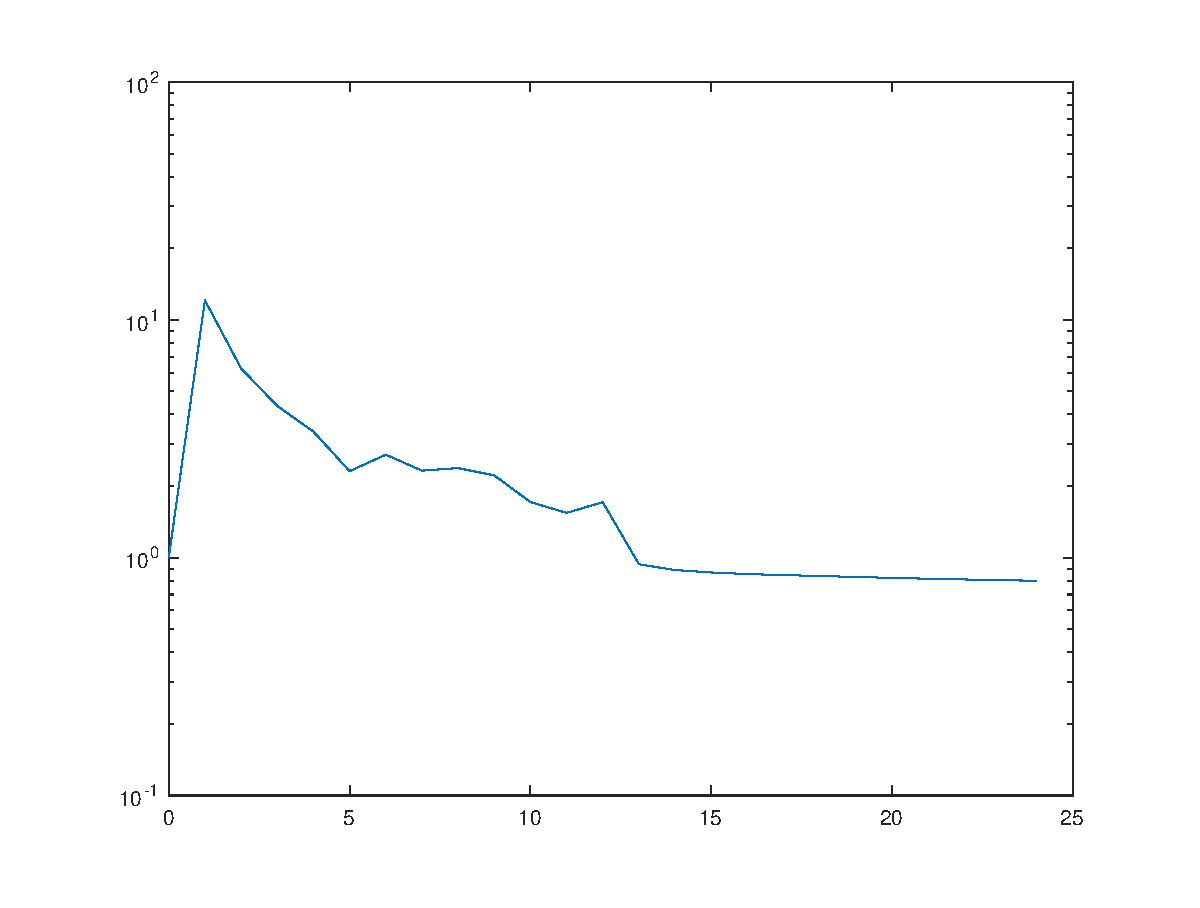
\includegraphics[scale=0.4]{7.eps}
\caption{svmHalfAvg}
\end{figure}

\subsection{Stochastic Average Gradient}
I write a program to implement the SAG algorithm (stochastic average gradient), which is a kind of stochastic subgradient method (proposed by Le Roux, Schmidt, and Bach, 2012).  The result is in Figure~8. Obviously, it performs much better than all the methods discussed above.
 
Codes of $svmSAG.m$ are in the Appendix.
\begin{figure}
\centering
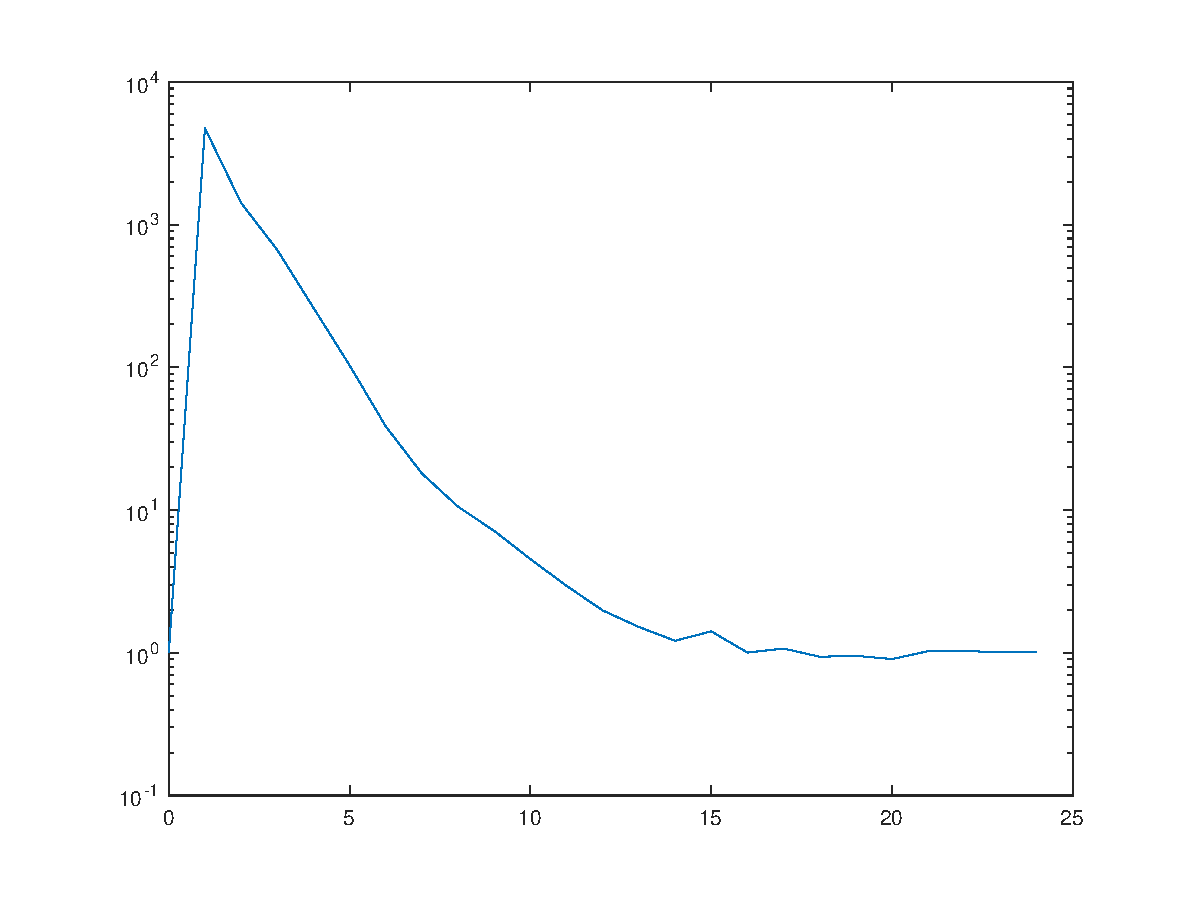
\includegraphics[scale=0.4]{8.eps}
\caption{svmSAG}
\end{figure}

\appendix
\section{Codes for Digit Classification}
\subsection{Codes for k-Nearest Neighbors}
\subsubsection{knn\_plot.m}
\begin{lstlisting}
% Edited by Yuanbo Han, 2017-11-14.

% Clear workspace.
clear all;
close all;

% Load data.
load ../data/mnist_train;
load ../data/mnist_valid;

N = size(valid_inputs, 1);
K = 1:2:9;  % set of values of k
num = length(K);  % the number of values of k

% Compute the classification rates for each k.
classification_rate = zeros(num, 1);
for i = 1:num
    valid_labels = run_knn( K(i), train_inputs, train_targets, valid_inputs);
    classification_rate(i) = sum(valid_labels == valid_targets) / N;
end

% Plot the classification rate against k.
figure;
plot(K, classification_rate, 'LineWidth', 2);
title('kNN for Validation Set', 'FontSize', 15);
xlabel('k', 'FontSize', 12);
ylabel('Classification rate', 'FontSize', 12);
set(gca, 'XTick', K);
set(gca, 'XTickLabel', K);

clear i;
\end{lstlisting}

\subsubsection{knn\_test.m}
\begin{lstlisting}
% Edited by Yuanbo Han, 2017-11-14.

% Clear workspace.
clear all;
close all;

% Load data.
load ../data/mnist_train;
load ../data/mnist_test;

N = size(test_inputs, 1);
k = 5;  % my chosen value of k
K = [k-2, k, k+2];

% Compute the classification rates for each k.
classification_rate = zeros(3, 1);
for i = 1:3
    test_labels = run_knn( K(i), train_inputs, train_targets, test_inputs);
    classification_rate(i) = sum(test_labels == test_targets) / N;
end

% Plot the classification rate against k.
figure;
plot(K, classification_rate, 'LineWidth', 2);
title('kNN for Test Set', 'FontSize', 15);
xlabel('k', 'FontSize', 12);
ylabel('Classification rate', 'FontSize', 12);
set(gca, 'XTick', K);
set(gca, 'XTickLabel', K);

clear i;
\end{lstlisting}

\subsection{Codes for Logistic Regression}
\subsubsection{logistic\_predict.m}
\begin{lstlisting}
function [y] = logistic_predict(weights, data)
% Compute the probabilities predicted by the logistic classifier.
%
% Note: N is the number of examples and
%       M is the number of features per example.
%
% Inputs:
%   weights:    (M+1) x 1 vector of weights, where the last element
%               corresponds to the bias (intercepts).
%   data:       N x M data matrix where each row corresponds
%               to one data point.
% Outputs:
%   y:          N x 1 vector of probabilities.
%               This is the output of the classifier.
%
% Yuanbo Han, 2017-11-12.

[N, ~] = size(data);
z = [data, ones(N,1)] * weights;
y = sigmoid(z);
end
\end{lstlisting}

\subsubsection{evaluate.m}
\begin{lstlisting}
function [ce, frac_correct] = evaluate(targets, y)
% Compute evaluation metrics.
% Inputs:
%   targets : N x 1 vector of binary targets. Values should be either 0 or 1.
%   y       : N x 1 vector of probabilities.
% Outputs:
%   ce           : (scalar) Cross entropy. CE(p, q) = E_p[-log q]. Here we
%                  want to compute CE(targets, y).
%   frac_correct : (scalar) Fraction of inputs classified correctly.
%
% Yuanbo Han, 2017-11-12.

ce = mean( - targets .* log(y) - (1-targets) .* log(1-y) );
frac_correct = ( sum(targets==1 & y>=0.5) + sum(targets==0 & y<0.5) ) / size(y,1);
end
\end{lstlisting}

\subsubsection{logistic.m}
\begin{lstlisting}
function [f, df, y] = logistic(weights, data, targets, ~)
% Calculate log likelihood and derivatives with respect to weights.
%
% Note: N is the number of examples and
%       M is the number of features per example.
%
% Inputs:
% 	weights:    (M+1) x 1 vector of weights, where the last element
%               corresponds to bias (intercepts).
% 	data:       N x M data matrix where each row corresponds
%               to one data point.
%	targets:    N x 1 vector of binary targets. Values should be either
%               0 or 1.
%   ~:          The hyperparameter structure is omitted.
%
% Outputs:
%	f:             The scalar error value (i.e. negative log likelihood).
%	df:            (M+1) x 1 vector of derivatives of error w.r.t. weights.
%   y:             N x 1 vector of probabilities.
%                  This is the output of the classifier.
%
% Yuanbo Han, 2017-11-12.

x = [ data, ones( size(data,1), 1 ) ];
z = x * weights;
y = sigmoid(z);
f = - z' * (targets - 1) - sum( log(y) );
df = - x' * ( targets - y );
end
\end{lstlisting}

\subsubsection{logistic\_pen.m}
\begin{lstlisting}
function [f, df, y] = logistic_pen(weights, data, targets, hyperparameters)
% Penalized logistic regression.
% Calculate log likelihood and derivatives with respect to weights.
%
% Note: N is the number of examples and
%       M is the number of features per example.
%
% Inputs:
% 	weights:    (M+1) x 1 vector of weights, where the last element
%               corresponds to bias (intercepts).
% 	data:       N x M data matrix where each row corresponds
%               to one data point.
%   targets:    N x 1 vector of targets class probabilities.
%   hyperparameters: The hyperparameter structure
%
% Outputs:
%	f:             The scalar error value (i.e. negative log liklihood
%                  + lambda/2 * weights(1:M)' * weights(1:M)).
%	df:            (M+1) x 1 vector of derivatives of error w.r.t. weights.
%   y:             N x 1 vector of probabilities.
%                  This is the output of the classifier.
%
% Yuanbo Han, 2017-11-13.

x = [ data, ones( size(data,1), 1 ) ];
z = x * weights;
y = sigmoid(z);
weights( length(weights) ) = 0;
f = - z' * (targets - 1) - sum( log(y) ) + hyperparameters.weight_regularization / 2 * weights' * weights;
df = - x' * ( targets - y ) + hyperparameters.weight_regularization * weights;
end
\end{lstlisting}

\subsubsection{plot\_cross\_entropy.m}
\begin{lstlisting}
% Edited by Yuanbo Han, 2017-11-12.

clear all;
close all;

%% Load data.
load ../data/mnist_train;
load ../data/mnist_train_small;
load ../data/mnist_valid;

%% Initialize hyperparameters.
% Learning rate
hyperparameters.learning_rate = 0.001;
% Weight regularization parameter
hyperparameters.weight_regularization = 0;
% Number of iterations
hyperparameters.num_iterations = 300;
% Logistic regression weights
% Set random weights.
weights = randn( (size(train_inputs,2) + 1), 1 );
%weights = zeros( (size(train_inputs,2) + 1), 1 );
weights_small = weights;

N = size(train_inputs, 1);
N_small = size(train_inputs_small, 1);

cross_entropy_train = zeros( hyperparameters.num_iterations, 1 );
cross_entropy_train_small = cross_entropy_train;
cross_entropy_valid = cross_entropy_train;
cross_entropy_valid_small = cross_entropy_train;

%% Begin learning with gradient descent.
for t = 1:hyperparameters.num_iterations
    
    % Find the negative log likelihood and derivatives w.r.t. weights.
    [f, df, predictions] = logistic(weights, ...
        train_inputs, ...
        train_targets, ...
        hyperparameters);
    
    [f_small, df_small, predictions_small] = logistic(weights_small, ...
        train_inputs_small, ...
        train_targets_small, ...
        hyperparameters);
    
    % Report the possible errors.
    if isnan(f) || isinf(f)
        error('f nan/inf error');
    end
    
    if isnan(f_small) || isinf(f_small)
        error('f_small nan/inf error');
    end
    
    % Find the cross entropy and fraction of correctly classified examples of training data.
    [cross_entropy_train(t), frac_correct_train] = evaluate(train_targets, predictions);
    [cross_entropy_train_small(t), frac_correct_train_small] = evaluate(train_targets_small, predictions_small);
    
    % Update weights.
    weights = weights - hyperparameters.learning_rate .* df;
    weights_small = weights_small - hyperparameters.learning_rate .* df_small;
    
    % Find the cross entropy and fraction of correctly classified examples of validation data.
    predictions_valid = logistic_predict(weights, valid_inputs);
    predictions_valid_small = logistic_predict(weights_small, valid_inputs);
    
    [cross_entropy_valid(t), frac_correct_valid] = evaluate(valid_targets, predictions_valid);
    [cross_entropy_valid_small(t), frac_correct_valid_small] = evaluate(valid_targets, predictions_valid_small);
    
    % Print some stats.
    fprintf(1, 'ITERATION:%4i   NLOGL:%11.2f TRAIN_CE:%16.6f TRAIN_FRAC:%12.2f VALIC_CE:%16.6f VALID_FRAC:%12.2f\n',...
        t, f/N, cross_entropy_train(t), frac_correct_train*100, cross_entropy_valid(t), frac_correct_valid*100);
    fprintf('%17sNLOGL_SMALL:%5.2f TRAIN_SMALL_CE:%10.6f TRAIN_SMALL_FRAC:%6.2f VALID_CE_SMALL:%10.6f VALID_FRAC_SMALL:%6.2f\n',...
        '', f_small/N_small, cross_entropy_train_small(t), frac_correct_train_small*100, cross_entropy_valid_small(t), frac_correct_valid_small*100);
    
end

%% Plot the cross entropy as training progresses.
figure;
subplot(1,2,1);
hold on;
title('mnist\_train', 'FontSize', 15);
plot(1:hyperparameters.num_iterations, cross_entropy_train, 'LineWidth', 2);
plot(1:hyperparameters.num_iterations, cross_entropy_valid, 'LineWidth', 2);
lgd = legend('train', 'valid', 'Location', 'NorthEast');
set(lgd, 'FontSize', 12);
xlabel('Iteration', 'FontSize', 12);
ylabel('Cross entropy', 'FontSize', 12);

subplot(1,2,2);
hold on;
title('mnist\_train\_small', 'FontSize', 15);
plot(1:hyperparameters.num_iterations, cross_entropy_train_small, 'LineWidth', 2);
plot(1:hyperparameters.num_iterations, cross_entropy_valid_small, 'LineWidth', 2);
lgd = legend('train\_small', 'valid', 'Location', 'NorthEast');
set(lgd, 'FontSize', 12);
xlabel('Iteration', 'FontSize', 12);
ylabel('Cross entropy', 'FontSize', 12);

clear t lgd;
\end{lstlisting}

\subsubsection{plot\_stats\_against\_lambda.m}
\begin{lstlisting}
% Edited by Yuanbo Han, 2017-11-13.

clear all;
close all;

%% Load data.
load ../data/mnist_train;
load ../data/mnist_train_small;
load ../data/mnist_valid;

%% Initialize hyperparameters.
% Learning rate
hyperparameters.learning_rate = 0.001;
% Number of iterations
hyperparameters.num_iterations = 300;

[N, M] = size(train_inputs);
[N_small, M_small] = size(train_inputs_small);

penalty_parameters = logspace(-3,0,4);  % values of penalty parameter
num = length(penalty_parameters);  % the number of values of penalty parameter

rerun_times = 10;

cross_entropy_train = zeros(rerun_times, num);
cross_entropy_train_small = zeros(rerun_times, num);
cross_entropy_valid = zeros(rerun_times, num);
cross_entropy_valid_small = zeros(rerun_times, num);

%% Compute some stats for each penalty parameters.
for i = 1:num
    hyperparameters.weight_regularization = penalty_parameters(i);
    for r = 1:rerun_times
        fprintf('\n\nPENALTY PARAMETER = %.3f   RUN TIME = %d\n\n', hyperparameters.weight_regularization, r);
        
        % Randomly initialize the logistic regression weights.
        weights = randn( M+1, 1 );
        weights_small = randn( M_small+1, 1 );
        
        % Begin learning with gradient descent.
        for t = 1:hyperparameters.num_iterations
            
            % Find the error value and derivatives w.r.t. weights.
            [f, df, predictions] = logistic_pen(weights, ...
                train_inputs, ...
                train_targets, ...
                hyperparameters);
            
            [f_small, df_small, predictions_small] = logistic_pen(weights_small, ...
                train_inputs_small, ...
                train_targets_small, ...
                hyperparameters);
            
            % Report the possible errors.
            if isnan(f) || isinf(f)
                error('f nan/inf error');
            end
            
            if isnan(f_small) || isinf(f_small)
                error('f_small nan/inf error');
            end
            
            % Find the cross entropy and fraction of correctly classified examples of training data.
            [cross_entropy_train(r,i), frac_correct_train(r,i)] = evaluate(train_targets, predictions);
            [cross_entropy_train_small(r,i), frac_correct_train_small(r,i)] = evaluate(train_targets_small, predictions_small);
            
            % Update weights.
            weights = weights - hyperparameters.learning_rate .* df;
            weights_small = weights_small - hyperparameters.learning_rate .* df_small;
            
            % Find the cross entropy and fraction of correctly classified examples of validation data.
            predictions_valid = logistic_predict(weights, valid_inputs);
            predictions_valid_small = logistic_predict(weights_small, valid_inputs);
            
            [cross_entropy_valid(r,i), frac_correct_valid(r,i)] = evaluate(valid_targets, predictions_valid);
            [cross_entropy_valid_small(r,i), frac_correct_valid_small(r,i)] = evaluate(valid_targets, predictions_valid_small);
            
            % Print some stats.
            fprintf(1, 'ITERATION:%4i   NLOGL:%11.2f TRAIN_CE:%16.6f TRAIN_FRAC:%12.2f VALIC_CE:%16.6f VALID_FRAC:%12.2f\n',...
                t, f/N, cross_entropy_train(r,i), frac_correct_train(r,i)*100, cross_entropy_valid(r,i), frac_correct_valid(r,i)*100);
            fprintf('%17sNLOGL_SMALL:%5.2f TRAIN_SMALL_CE:%10.6f TRAIN_SMALL_FRAC:%6.2f VALID_CE_SMALL:%10.6f VALID_FRAC_SMALL:%6.2f\n',...
                '', f_small/N_small, cross_entropy_train_small(r,i), frac_correct_train_small(r,i)*100, cross_entropy_valid_small(r,i), frac_correct_valid_small(r,i)*100);
            
        end
    end
end

%% Plot the cross entropy and classification rate against penalty parameters.
figure;
subplot(2,2,1);
hold on;
title('mnist\_train', 'FontSize', 15);
plot(1:num, mean(cross_entropy_train, 1), 'LineWidth', 2);
plot(1:num, mean(cross_entropy_valid, 1), 'LineWidth', 2);
lgd = legend('train', 'valid', 'Location', 'NorthEast');
set(lgd, 'FontSize', 12);
xlabel('\lambda', 'FontSize', 12);
ylabel('Cross entropy', 'FontSize', 12);
set(gca, 'XTick', 1:num);
set(gca, 'XTickLabel', penalty_parameters);

subplot(2,2,2);
hold on;
title('mnist\_train', 'FontSize', 15);
plot(1:num, mean(frac_correct_train, 1), 'LineWidth', 2);
plot(1:num, mean(frac_correct_valid, 1), 'LineWidth', 2);
lgd = legend('train', 'valid', 'Location', 'NorthEast');
set(lgd, 'FontSize', 12);
xlabel('\lambda', 'FontSize', 12);
ylabel('Classification rate', 'FontSize', 12);
set(gca, 'XTick', 1:num);
set(gca, 'XTickLabel', penalty_parameters);

subplot(2,2,3);
hold on;
title('mnist\_train\_small', 'FontSize', 15);
plot(1:num, mean(cross_entropy_train_small, 1), 'LineWidth', 2);
plot(1:num, mean(cross_entropy_valid_small, 1), 'LineWidth', 2);
lgd = legend('train\_small', 'valid', 'Location', 'NorthEast');
set(lgd, 'FontSize', 12);
xlabel('\lambda', 'FontSize', 12);
ylabel('Cross entropy', 'FontSize', 12);
set(gca, 'XTick', 1:num);
set(gca, 'XTickLabel', penalty_parameters);

subplot(2,2,4);
hold on;
title('mnist\_train\_small', 'FontSize', 15);
plot(1:num, mean(frac_correct_train_small, 1), 'LineWidth', 2);
plot(1:num, mean(frac_correct_valid_small, 1), 'LineWidth', 2);
lgd = legend('train\_small', 'valid', 'Location', 'NorthEast');
set(lgd, 'FontSize', 12);
xlabel('\lambda', 'FontSize', 12);
ylabel('Classification rate', 'FontSize', 12);
set(gca, 'XTick', 1:num);
set(gca, 'XTickLabel', penalty_parameters);

clear i r t lgd;
\end{lstlisting}

\subsection{Codes for Naive Bayes}
\subsubsection{train\_nb.m}
\begin{lstlisting}
function [log_prior, class_mean, class_var] = train_nb(train_data, train_label)
% TRAIN_NB trains a Naive Bayes binary classifier. All conditional
% distributions are Gaussian.
%
% Usage:
%   [log_prior, class_mean, class_var] = train_nb(train_data, train_label);
%
% Inputs:
%   train_data  : n_examples x n_dimensions matrix
%   train_label : n_examples x 1 binary label vector
%
% Outputs:
%   log_prior   : 2 x 1 vector, log_prior(i) = log(p(C=i)).
%   class_mean  : 2 x n_dimensions matrix, class_mean(i,:) is the mean
%                 vector for class i.
%   class_var   : 2 x n_dimensions matrix, class_var(i,:) is the variance
%                 vector for class i.
%
% Modified by Yuanbo Han, 2017-11-14: Omit the unused variable by '~', and
%                                     correct the comments.

SMALL_CONSTANT = 1e-10;

[~, n_dims] = size(train_data);
K = 2;

prior = zeros(K, 1);
class_mean = zeros(K, n_dims);
class_var = zeros(K, n_dims);

for k = 1 : K
    prior(k) = mean(train_label == (k-1));
    class_mean(k, :) = mean(train_data(train_label == (k-1), :), 1);
    class_var(k, :) = var(train_data(train_label == (k-1), :), 0, 1);
end

class_var = class_var + SMALL_CONSTANT;
log_prior = log(prior + SMALL_CONSTANT);

end
\end{lstlisting}

\subsubsection{test\_nb.m}
\begin{lstlisting}
function [prediction, accuracy] = test_nb(test_data, test_label, log_prior, class_mean, class_var)
% TEST_NB tests a learned Naive Bayes classifier.
%
% Usage:
%   [prediction, accuracy] = test_nb(test_data, test_label, log_prior, ...
%   class_mean, class_var);
%
% Inputs:
%   test_data  : n_examples x n_dimensions matrix
%   test_label : n_examples x 1 binary label vector
%   log_prior  : 2 x 1 vector, log_prior(i) = log(p(C=i)).
%   class_mean : 2 x n_dimensions matrix, class_mean(i,:) is the mean
%                vector for class i.
%   class_var  : 2 x n_dimensions matrix, class_var(i,:) is the variance
%                vector for class i.
%
% Outputs:
%   prediction : n_examples x 1 binary label vector
%   accuracy   : a real number
%
% Modified by Yuanbo Han, 2017-11-14: Correct the comments.

K = length(log_prior);
n_examples = size(test_data, 1);

log_prob = zeros(n_examples, K);

for k = 1 : K
    mean_mat = repmat(class_mean(k, :), [n_examples, 1]);
    var_mat = repmat(class_var(k, :), [n_examples, 1]);
    log_prob(:, k) = sum(-0.5 * (test_data - mean_mat).^2 ./ var_mat - 0.5 * log(var_mat), 2) + log_prior(k);
end

[~, prediction] = max(log_prob, [], 2);
prediction = prediction - 1;
accuracy = mean(prediction == test_label);

end
\end{lstlisting}

\subsubsection{run\_nb.m}
\begin{lstlisting}
% Learn a Naive Bayes classifier on the digit dataset, evaluate its
% performance on training and test sets, then visualize the mean and
% variance for each class.
% Edited by Yuanbo Han, 2017-11-14.

% Clear workspace and close figures.
clear all;
close all;

% Load data.
load ../data/mnist_train;
load ../data/mnist_test;

% Add your code here (it should be less than 10 lines).
[log_prior, class_mean, class_var] = train_nb(train_inputs, train_targets);
[prediction_train, accuracy_train] = test_nb(train_inputs, train_targets, log_prior, class_mean, class_var);
[prediction_test, accuracy_test] = test_nb(test_inputs, test_targets, log_prior, class_mean, class_var);

fprintf('Training accuracy = %5.2f%%\n', accuracy_train * 100);
fprintf('Test accuracy = %9.2f%%\n', accuracy_test * 100);

plot_digits(class_mean);  % mean visualization
plot_digits(class_var);  % variance visualization
\end{lstlisting}

\section{Codes for Stochastic Subgradient Methods}
\subsection{svmAvg.m}
\begin{lstlisting}
function [model] = svmAvg(X,y,lambda,maxIter)
% SVMAVG minimizes the SVM objective function by stochastic method based on
% the running average of w.
%
% Yuanbo Han, 2017-11-18.

% Add the bias variable.
[n,d] = size(X);
X = [ones(n,1), X];

% Use the transpose to accelerate the program.
Xt = X';

% Initialize the values of regression parameters.
w = zeros(d+1,1);

% The running average of w
w_bar = w;

% Apply stochastic method based on the running average of w.
for t = 1:maxIter
    if mod(t-1,n) == 0
        % Plot our progress.
        % (turn this off for acceleration)
        
        objValues(1+(t-1)/n) = (1/n)*sum(max(0,1-y.*(X*w_bar))) + (lambda/2)*(w_bar'*w_bar);
        semilogy([0:t/n],objValues);
        pause(.1);
    end
    
    % Pick a random training example.
    i = randi(n);
    
    % Compute the i-th subgradient.
    [~, sg] = hingeLossSubGrad(w,Xt,y,i);
    
    % Set step size.
    alpha = 1 / (lambda * t);
    
    % Take stochastic subgradient step.
    w = w - alpha * (sg + lambda * w);
    
    % Renew the running average of w.
    w_bar = (t-1)/t * w_bar + 1/t * w;
end

model.w = w_bar;
model.predict = @predict;

end

function [yhat] = predict(model,Xhat)
d = size(Xhat,1);
Xhat = [ones(d,1), Xhat];
w = model.w;
yhat = sign(Xhat * w);
end

function [f,sg] = hingeLossSubGrad(w,Xt,y,i)
% Function value
wtx = w' * Xt(:,i);
f = max(0, 1 - y(i) * wtx );

% Subgradient
if f > 0
    sg = - y(i) * Xt(:,i);
else
    sg = zeros(size(Xt,1), 1);
end

end
\end{lstlisting}

\subsection{svmHalfAvg.m}
\begin{lstlisting}
function [model] = svmHalfAvg(X,y,lambda,maxIter)
% SVMAVG minimizes the SVM objective function by stochastic gradient
% method, based on the current w for the first half iterations, and based
% on the running average of w for the second half.
%
% Yuanbo Han, 2017-11-18.

% Add the bias variable.
[n,d] = size(X);
X = [ones(n,1), X];

% Use the transpose to accelerate the program.
Xt = X';

% Initialize the values of regression parameters.
w = zeros(d+1,1);

% The 1st half: based on the current w

% Apply stochastic gradient method.
for t = 1 : (maxIter/2)
    if mod(t-1,n) == 0
        % Plot our progress.
        % (turn this off for acceleration)
        
        objValues(1+(t-1)/n) = (1/n)*sum(max(0,1-y.*(X*w))) + (lambda/2)*(w'*w);
        semilogy([0:t/n],objValues);
        pause(.1);
    end
    
    % Pick a random training example.
    i = randi(n);
    
    % Renew the i-th and the average subgradient.
    [~, sg] = hingeLossSubGrad(w,Xt,y,i);
    
    % Set step size.
    alpha = 1 / (lambda * t);
    
    % Take stochastic subgradient step.
    w = w - alpha * ( sg + lambda * w );
end

% The 2nd half: based on the running average of w

% The running average of w
w_bar = w;

% Apply stochastic method based on the running average of w.
k = 1;
for t = ceil(maxIter/2) : maxIter
    if mod(t-1,n) == 0
        % Plot our progress.
        % (turn this off for acceleration)
        
        objValues(1+(t-1)/n) = (1/n)*sum(max(0,1-y.*(X*w_bar))) + (lambda/2)*(w_bar'*w_bar);
        semilogy([0:t/n],objValues);
        pause(.1);
    end
    
    % Pick a random training example.
    i = randi(n);
    
    % Compute the i-th subgradient.
    [~, sg] = hingeLossSubGrad(w,Xt,y,i);
    
    % Set step size.
    alpha = 1 / (lambda * t);
    
    % Take stochastic subgradient step.
    w = w - alpha * (sg + lambda * w);
    
    % Renew the running average of w.
    w_bar = (k-1)/k * w_bar + 1/k * w;
    k = k + 1;
end

model.w = w_bar;
model.predict = @predict;

end

function [yhat] = predict(model,Xhat)
d = size(Xhat,1);
Xhat = [ones(d,1), Xhat];
w = model.w;
yhat = sign(Xhat * w);
end

function [f,sg] = hingeLossSubGrad(w,Xt,y,i)
% Function value
wtx = w' * Xt(:,i);
f = max(0, 1 - y(i) * wtx );

% Subgradient
if f > 0
    sg = - y(i) * Xt(:,i);
else
    sg = zeros(size(Xt,1), 1);
end

end
\end{lstlisting}

\subsection{svmSAG.m}
\begin{lstlisting}
function [model] = svmSAG(X,y,lambda,maxIter)
% SVMAVG minimizes the SVM objective function by stochastic average
% gradient (SAG) method.
%
% Yuanbo Han, 2017-11-18.

% Add the bias variable.
[n,d] = size(X);
X = [ones(n,1), X];

% Use the transpose to accelerate the program.
Xt = X';

% Initialize the values of regression parameters.
w = zeros(d+1,1);

% Compute the initial subgradients.
sg = zeros(d+1,n);
for j=1:n
    sg(:,j) = - y(j) * Xt(:,j);
end

% The average subgradient
m = mean(sg, 2);

% Apply stochastic average gradient (SAG) method.
for t = 1:maxIter
    if mod(t-1,n) == 0
        % Plot our progress.
        % (turn this off for acceleration)
        
        objValues(1+(t-1)/n) = (1/n)*sum(max(0,1-y.*(X*w))) + (lambda/2)*(w'*w);
        semilogy([0:t/n],objValues);
        pause(.1);
    end
    
    % Pick a random training example.
    i = randi(n);
    
    % Compute the i-th subgradient, and renew the average subgradient.
    m = m - sg(:,i) / n;
    [~, sg(:,i)] = hingeLossSubGrad(w,Xt,y,i);
    m = m + sg(:,i) / n;
    
    % Set step size.
    alpha = 1 / (lambda * t);
    
    % Take stochastic subgradient step.
    w = w - alpha * ( m + lambda * w );
end

model.w = w;
model.predict = @predict;

end

function [yhat] = predict(model,Xhat)
d = size(Xhat,1);
Xhat = [ones(d,1), Xhat];
w = model.w;
yhat = sign(Xhat * w);
end

function [f,sg] = hingeLossSubGrad(w,Xt,y,i)
% Function value
wtx = w' * Xt(:,i);
f = max(0, 1 - y(i) * wtx );

% Subgradient
if f > 0
    sg = - y(i) * Xt(:,i);
else
    sg = zeros(size(Xt,1), 1);
end

end
\end{lstlisting}

\end{document}